\section{Recursive Algebraic Data Types}
\noindent
We've been working with primitive data types like integers, floats, and strings. But what if we want to create our own data types?

\begin{Def}[Algebraic Data Types (ADT)]

    Algebraic Data Types (\texttt{ADT}) are a way to define new data types by combining existing types using \textbf{sum} (variant) and \textbf{product} (tuple/record) constructions.
\end{Def}

\begin{Example}[Primitive Types vs. ADTs]

    In \texttt{OCaml}, some data types are primitive, while others are constructed using \textbf{ADTs}.

    \begin{lstlisting}[language=OCaml, caption={Primitive Types vs. ADTs}, numbers=none]
    (* Primitive types (Not ADTs) *)
    let x : int = 42      (* int is a built-in type *)
    let y : bool = true   (* bool is a built-in type *)

    (* Algebraic Data Types (ADTs) *)

    (* Sum type (Variant) *)
    type shape =
      | Circle of float
      | Rectangle of float * float
    
    (* Product type (Record) *)
    type point = { x: float; y: float }
    \end{lstlisting}

    \noindent
    Here, \texttt{int} and \texttt{bool} are \textbf{primitive types}, meaning they exist independently. In contrast:
    \begin{itemize}
        \item The \texttt{shape} type is a \textbf{sum type (variant)}, an ADT where a value can be either a \texttt{Circle} or a \texttt{Rectangle}.
        \item The \texttt{point} type is a \textbf{product type (record)}, an ADT that groups multiple values together.
    \end{itemize}
\end{Example}

\newpage 

\subsection{Recursive Types}
\noindent
ADTs can be recursive, meaning they can refer to themselves in their definition. This allows the creation of data structures with variable lengths.
\begin{theo}[Recursive ADTs and Variable-Length Data]

    Consider the following recursive definition of a list in \texttt{OCaml}:
    
    \begin{lstlisting}[language=OCaml, caption={Recursive List Definition}, numbers=none]
    type intlist =
        | Nil
        | Cons of int * intlist

    let example = Cons (1, Cons (2, Cons (3, Nil)))
    \end{lstlisting}
\end{theo}

\noindent
Consider the following illustration:
\begin{figure}[h]
    \hspace{-1em}
    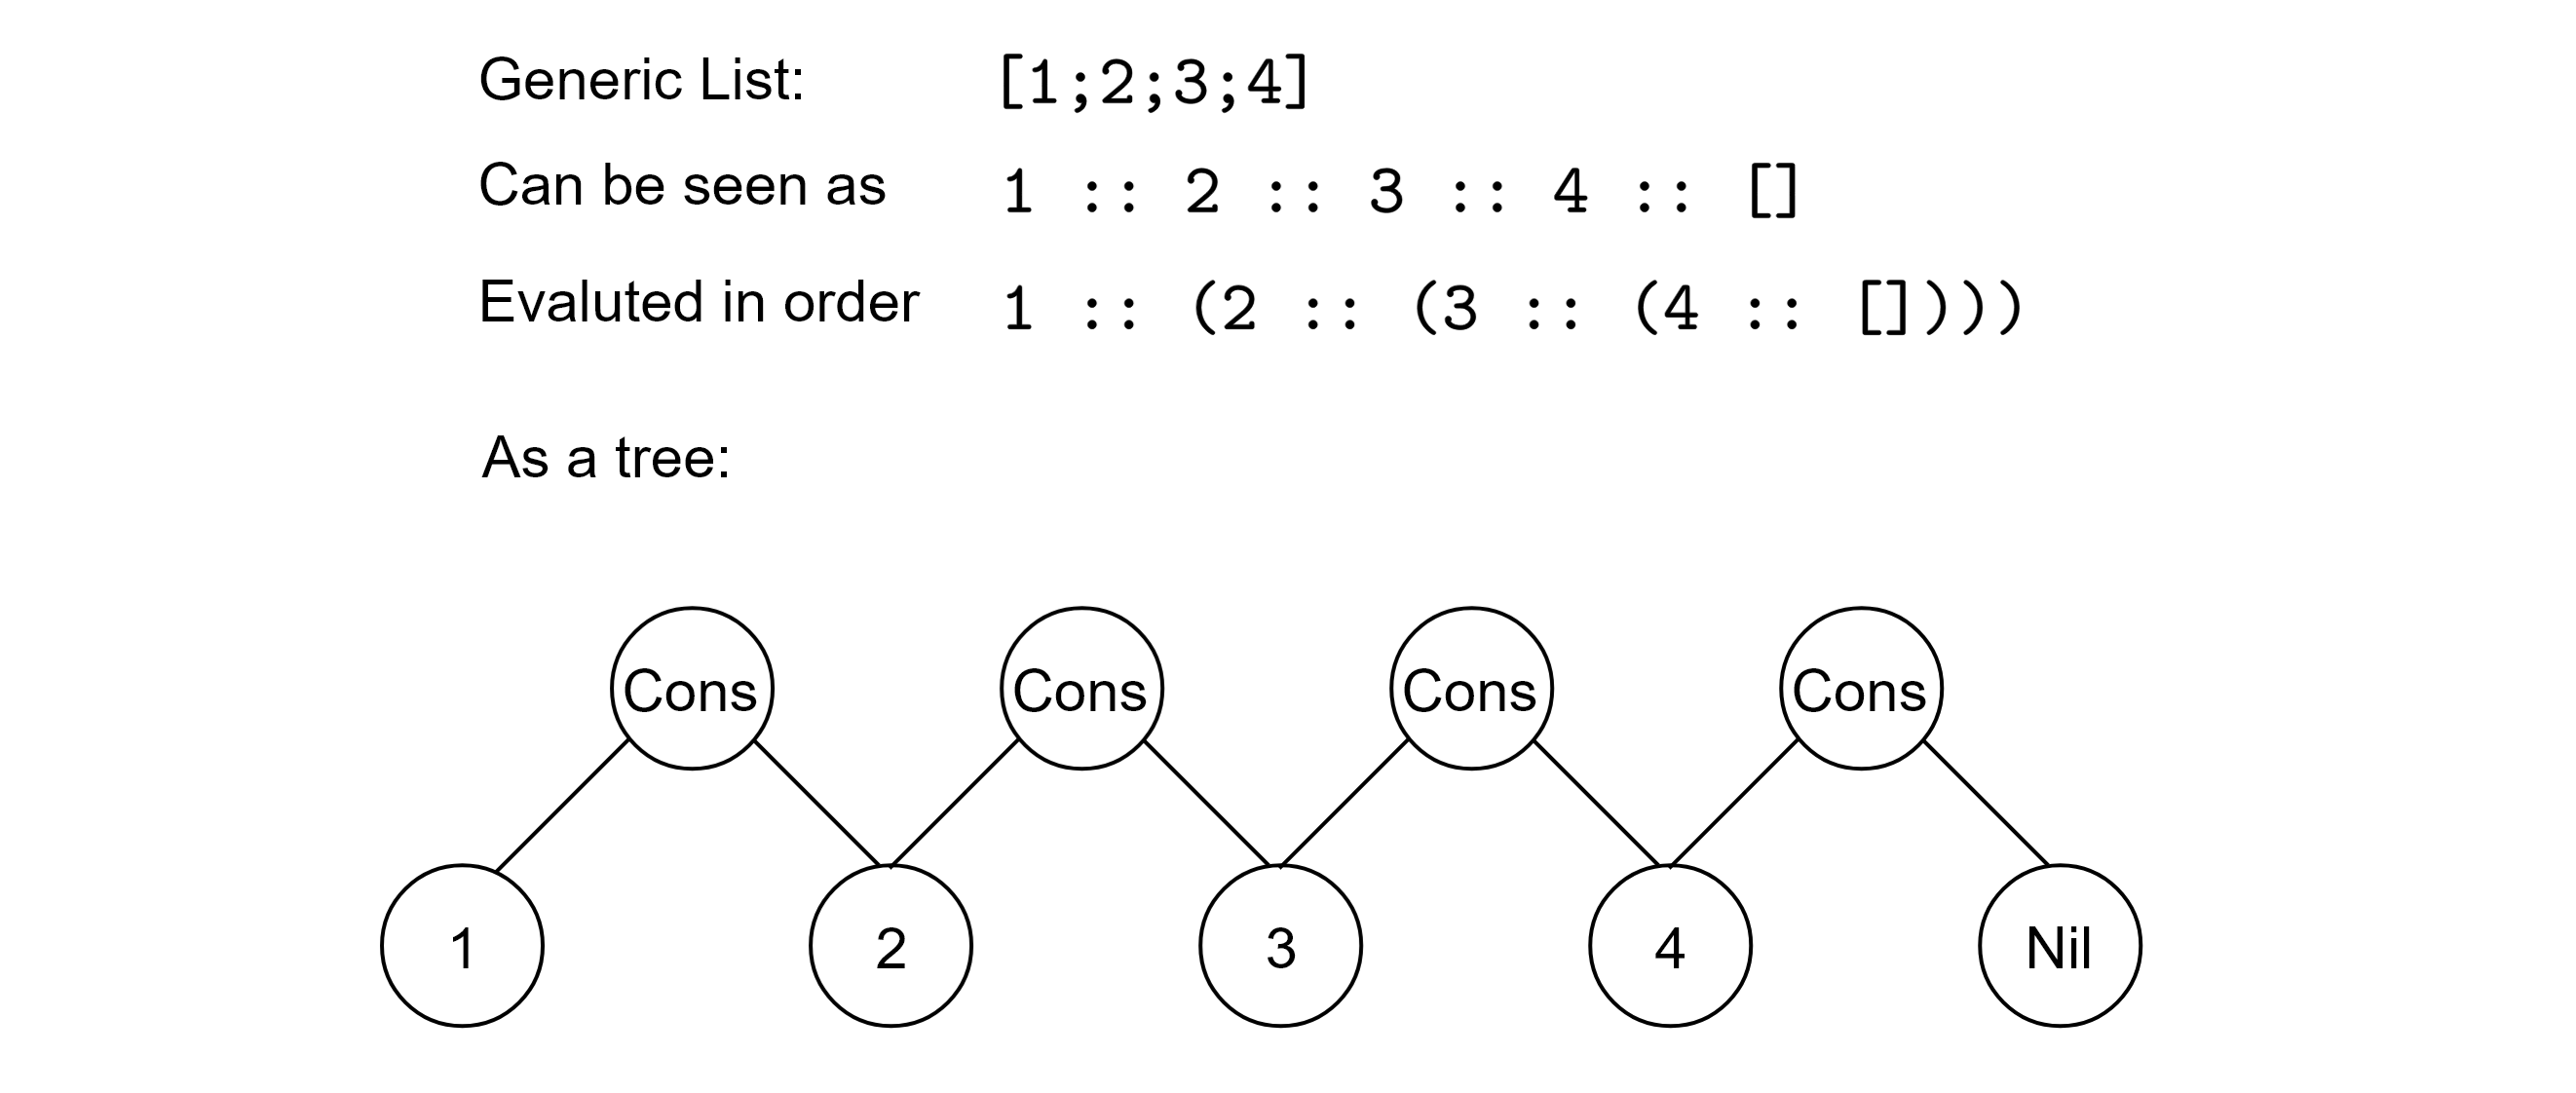
\includegraphics[width=1.1\textwidth]{Sections/adt/cons.png}
    \caption{Ocaml list representations.}
\end{figure}

\noindent
We can represent this of an integer list as either being,
\begin{itemize}
    \item \textbf{Base case}: Empty (\snippet{Nil})
    \item \textbf{Recursive case}: An Integer entry with reference to another entry (\snippet{int * intlist}), for which we label \snippet{Cons}.
\end{itemize}

\noindent
In essence, a list is actually a type of tree structure, where each node has a value and a reference to the next node. And that in reality, we may 
represent lists, trees, and graphs as an Algebraic Data Type.

\newpage 

\noindent
For instance, binary tree traversal can be represented as follows:

\begin{Example}
    We can define a binary tree as a recursive \texttt{ADT} in \texttt{OCaml}, where each node contains a value and references to left and right subtrees.

    \begin{lstlisting}[language=OCaml, caption={Binary Tree Definition and Traversals}, numbers=none]
    (* Define a binary tree type *)
    type 'a btree =
      | Empty
      | Node of 'a * 'a btree * 'a btree

    (* Example tree *)
    let example_tree =
      Node (1,
        Node (2, Node (4, Empty, Empty), Node (5, Empty, Empty)),
        Node (3, Node (6, Empty, Empty), Node (7, Empty, Empty))
      )

    (* Preorder traversal: Root -> Left -> Right *)
    let rec preorder t =
      match t with
      | Empty -> []
      | Node (v, left, right) -> [v] @ preorder left @ preorder right

    (* Inorder traversal: Left -> Root -> Right *)
    let rec inorder t =
      match t with
      | Empty -> []
      | Node (v, left, right) -> inorder left @ [v] @ inorder right

    (* Postorder traversal: Left -> Right -> Root *)
    let rec postorder t =
      match t with
      | Empty -> []
      | Node (v, left, right) -> postorder left @ postorder right @ [v]

    (* Example usage *)
    let _ =
      let pre = preorder example_tree in
      let inord = inorder example_tree in
      let post = postorder example_tree in
      (pre, inord, post) 
    (* Outputs: 
    ([1; 2; 4; 5; 3; 6; 7], [4; 2; 5; 1; 6; 3; 7], [4; 5; 2; 6; 7; 3; 1])
    *)
    \end{lstlisting}
\end{Example}

\newpage 

\noindent
We may use recursive ADTs to model expressions. Take for instance a basic arithmetic expression:
\begin{figure}[h]
    \centering
    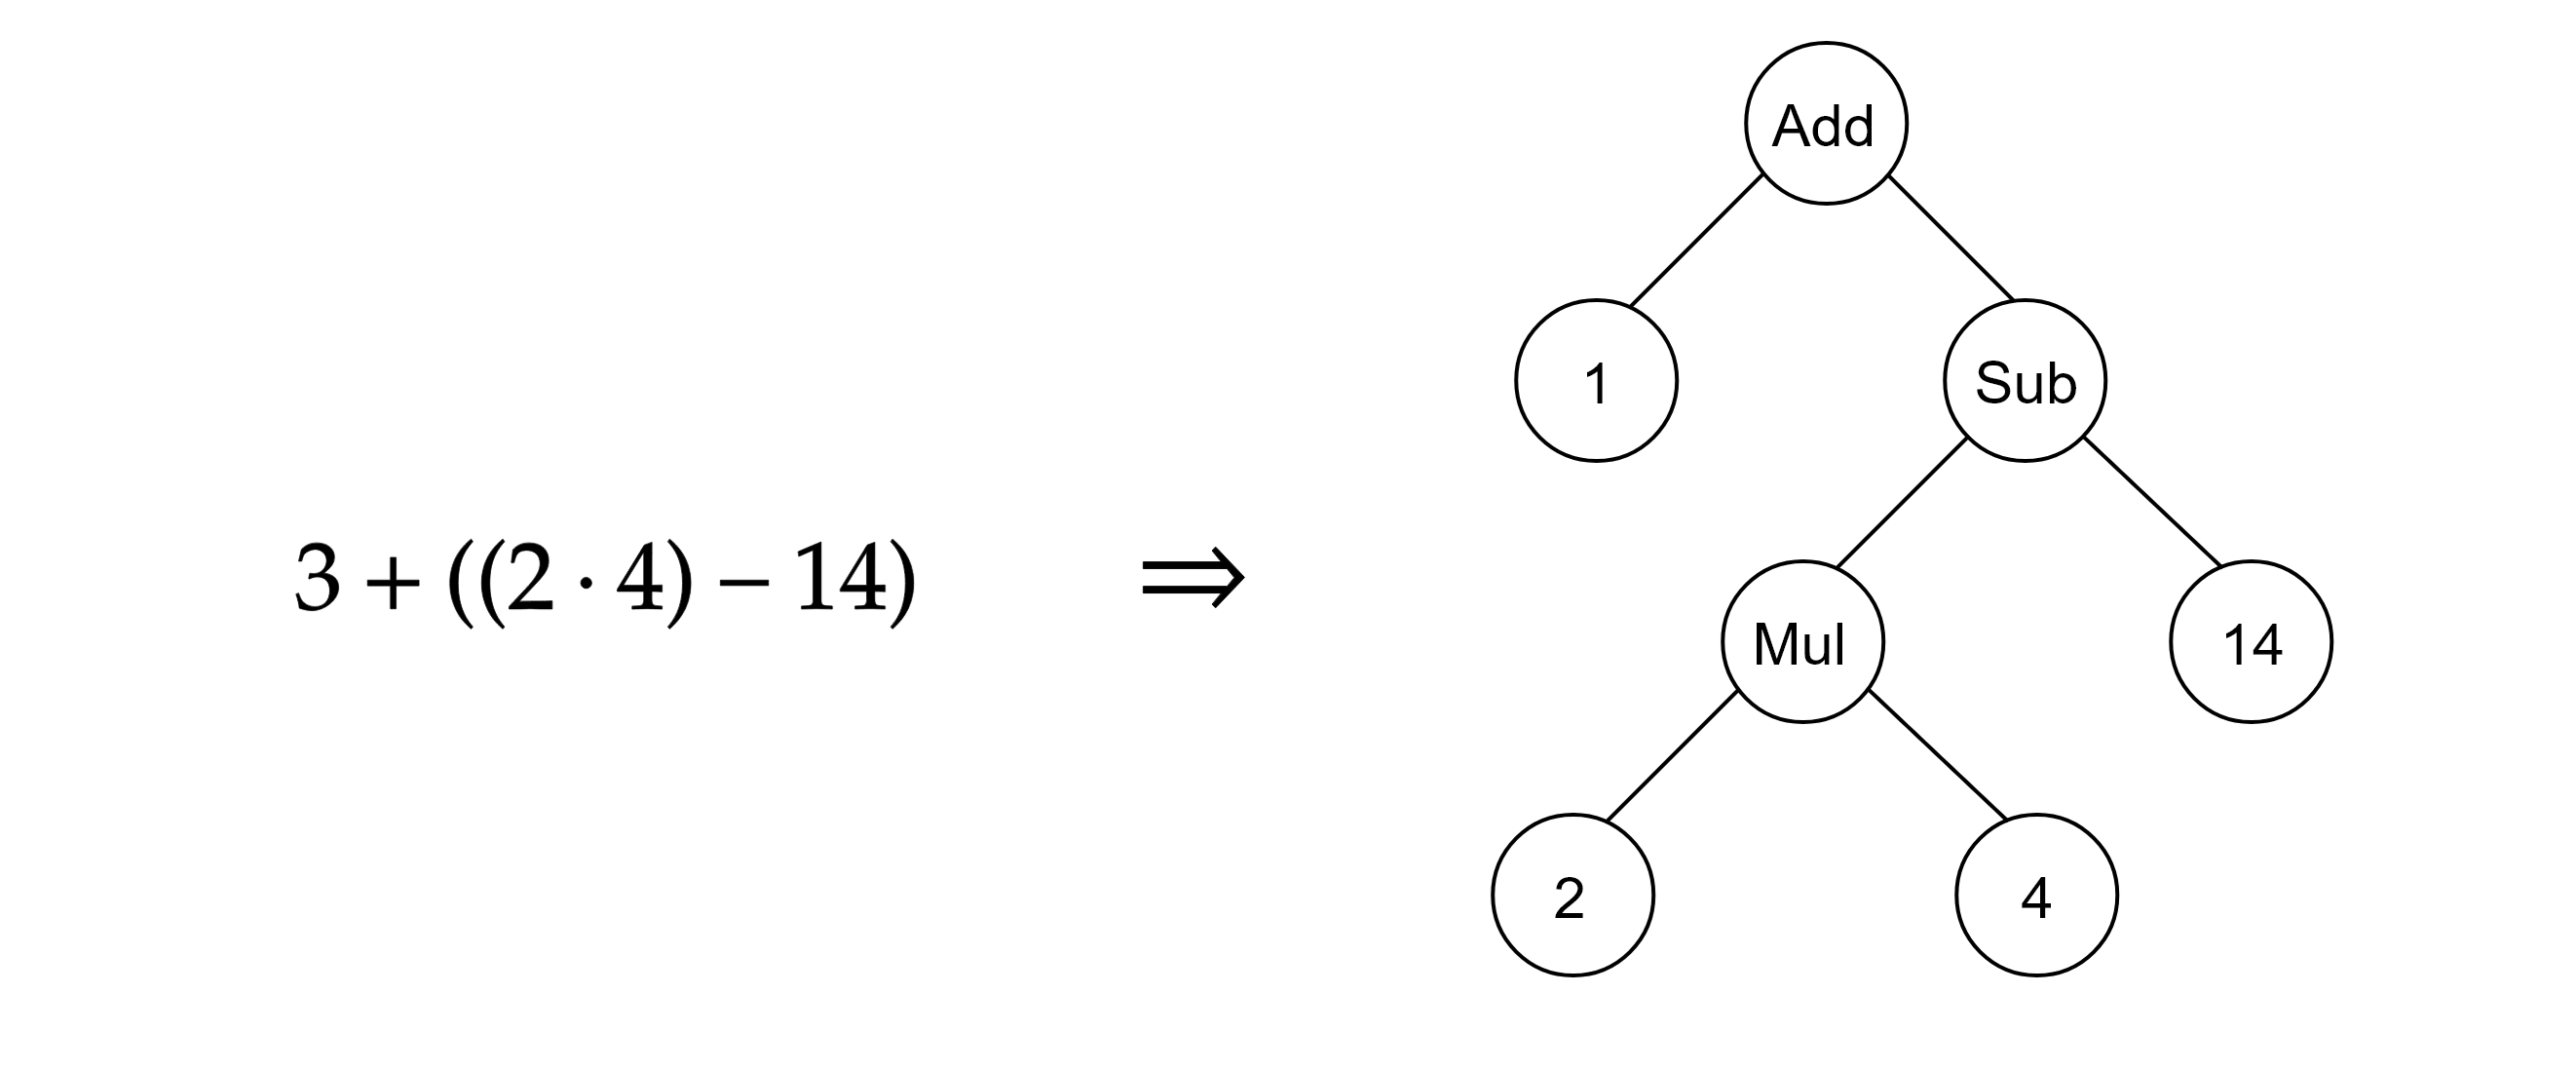
\includegraphics[width=1\textwidth]{Sections/adt/expr.png}
    \caption{Arithmetic expression tree.}
\end{figure}

\vspace{-1em}
\begin{Example}[Arithmetic Data Type]

    We define an arithmetic data type for Addition, Multiplication, and Subtraction of integers:
    \begin{lstlisting}[language=OCaml, caption={Arithmetic Expression Definition}, numbers=none]
    type expr =
      | Num of int
      | Add of expr * expr
      | Mul of expr * expr
      | Sub of expr * expr
    
    let _ = Add (Val 3, Sub (Mul (Val 2, Val 4), Val 14))
    (* Renders:      3 + ((2 * 4) - 14)                *)
    \end{lstlisting}
\end{Example}

\subsection{Parametric \& Polymorphic Types}
\noindent
Now what if we want to create a generic list that can store any type of value? In this case, we must parametrize the type definition.
\begin{Def}[Parametric Types]

    Parametric types are types that can take one or more type parameters. They are useful for creating generic data structures that can store values of any type.
\end{Def}

\newpage 

\begin{Example}[Parametric List]

    We can define a parametric list in \texttt{OCaml} that can store values of any type:
    \begin{lstlisting}[language=OCaml, caption={Parametric List Definition}, numbers=none]
    type 'a list =
      | Nil
      | Cons of 'a * 'a list

    let example_ints = Cons (1, Cons (2, Cons (3, Nil)))
    let example_strings = Cons ("a", Cons ("b", Cons ("c", Nil)))
    \end{lstlisting}

    \noindent
    Where \snippet{'a} is a type parameter and \snippet{list} is the type constructor.
\end{Example}

\noindent
Making the type generic also makes it polymorphic, meaning it can store values of any type. This is useful for creating reusable data structures.
\begin{Def}[Polymorphic Types]

    \textbf{Polymorphism} is the ability of a function or data type to operate on values of different types. \textbf{Parametric polymorphism} refers to functions or data types that are generic and can operate on values of any type.
\end{Def}

There is no overloading on types in \texttt{OCaml}:
\begin{Def}[Ad-Hoc Polymorphism]

    \textbf{Ad-hoc polymorphism} refers to a type of polymorphism where a function can be defined multiple times with different type signatures, allowing it to operate on different types using \textit{distinct implementations}.

    Some languages, such as C++ (via function overloading) and Haskell (via type classes), support ad-hoc polymorphism. However, \textbf{OCaml does not support ad-hoc polymorphism} because function overloading is not allowed—redefining a function replaces the previous definition.\\
    \begin{lstlisting}[language=OCaml, caption={No Overloading in OCaml}, numbers=none]
    (* The following isn't possible *)
    let add (a : int) (b : int) : int = a + b
    let add (a : string) (b : string) : string = a ^ b (* Overwrite *)
    let add (a : 'a list) (b : 'a list) : 'a list = a @ b (* Overwrites *)
    \end{lstlisting}
\end{Def}

\newpage 

\begin{Tip} Tony Hoare calls his invention of the
null pointer a ``billion-dollar mistake''
OCaml doesn't have null pointers\\
\noindent
\rule{\textwidth}{0.4pt}
\textit{I call it my billion-dollar mistake. It was the invention of the null
reference in 1965. At that time, I was designing the first comprehensive type
system for references in an object oriented language (ALGOL W). My goal was to
ensure that all use of references should be absolutely safe, with checking
performed automatically by the compiler. But I couldn't resist the temptation
to put in a null reference, simply because it was so easy to implement. This
has led to innumerable errors, vulnerabilities, and system crashes, which have
probably caused a billion dollars of pain and damage in the last forty years.}\\
-- Tony Hoare, inventor of null pointers
\end{Tip}

